%%%%%%%%%%%%%%%%%%%%%%%%%%%%%%%%%%%%%%%%%%%%%%%%%%%%
%    Harvard Data Science Review Latex Template    %
%%%%%%%%%%%%%%%%%%%%%%%%%%%%%%%%%%%%%%%%%%%%%%%%%%%%

\documentclass[]{hdsr}

%Graphics should all go in the figs/ directory
\graphicspath{{figs/}}

\usepackage{amsmath}
\usepackage{commath}
\usepackage{graphicx}

\usepackage{listings}
\usepackage{color} %red, green, blue, yellow, cyan, magenta, black, white
\definecolor{mygreen}{RGB}{28,172,0} % color values Red, Green, Blue
\definecolor{mylilas}{RGB}{170,55,241}

\begin{document}

\lstset{language=Matlab,%
    %basicstyle=\color{red},
    breaklines=true,%
    morekeywords={matlab2tikz},
    keywordstyle=\color{blue},%
    morekeywords=[2]{1}, keywordstyle=[2]{\color{black}},
    identifierstyle=\color{black},%
    stringstyle=\color{mylilas},
    commentstyle=\color{mygreen},%
    showstringspaces=false,%without this there will be a symbol in the places where there is a space
    numbers=left,%
    numberstyle={\tiny \color{black}},% size of the numbers
    numbersep=9pt, % this defines how far the numbers are from the text
    emph=[1]{for,end,break},emphstyle=[1]\color{red}, %some words to emphasise
    %emph=[2]{word1,word2}, emphstyle=[2]{style},    
}

% Larger bottom margin for the first page
\newgeometry{bottom=1.5in}

% Editorial staff will replace the following values:
% 1. Volume number
% 2. Issue number
% 3. Article DOI
% e.g. for Volume 2, Issue 3, DOI 12.345:
% \volumeheader{2}{3}{12.345}
%\volumeheader{0}{0}{00.000}

\begin{center}

  \title{Path Integral Stochastic Optimal Control for Dynamic System: Swing-up Task}
  \maketitle

  % Start page numbering on second page. Must appear *after* \maketitle
  \thispagestyle{empty}
  
  \vspace*{.2in}

  % Authors and Affiliations
  \begin{tabular}{cc}
    Erivelton Gualter dos Santos\upstairs{\affilone,*}, Hamed Kayello\upstairs{\affilone}
   \\[0.25ex]
   {\small \upstairs{\affilone} Ph.D Candidate, Cleveland State University} \\
   {\small \upstairs{\affiltwo} Ph.D, Instructor, Cleveland State Univrsity} \\
  \end{tabular}
  
  % Replace with corresponding author email address
  \emails{
    \upstairs{*}erivelton.gualter@gmail.com
    }
  \vspace*{0.4in}

%\begin{abstract}
%The abstract should be no more than 250 words.
%\end{abstract}
\end{center}

\vspace*{0.15in}

\section{Dynamic Representation of Stochastic System}
\label{sec1}

According to \citet{morrison2012art}, \textit{``modeling is neither science nor mathematics; it is the craft that builds bridges between the two.''} It is an essential tool for mathematically describe a device's behavior that can be computed and compared to the system's measured information. In system dynamics and robotics, differential equations have significantly been used for this task and showed success in describing these behaviors \citep{karnopp2012system,meriam2012engineering}. However, ``unpredictable'' states are not considered in many of these tools, bringing false models.

Deterministic dynamical mathematical models by themselves are not sufficient to map the system's randomness because these random variables are exogenous. It boils down to the fact that the perturbation to the state variables is independent \citep{morrison2012art}.  To mitigate this problem, studying the stochastic system has shed light on the robotic system's field. Last, the class of stochastic systems englobes both continuous and discrete systems.  Along with this work, modeling and control are performed in the discrete domain. 

\subsection{Deterministic vs. Stochastic System}

Deterministic representation of a model assumes it can predict all the states of a system. However, it is not accurate to practical applications that present uncertain parameters or disturbances \citep{skogestad2007multivariable}. To initiate the discussion of stochastic system control formulation, consider the continuous-time dynamic in the following:

\begin{equation}
    \dot{x} = f(t,x,u) \label{eq:ss_cont}
\end{equation}

Equation \ref{eq:ss_cont} is a mathematical formulation mapping from a set of variables into another, where the control input $u$ is the action in the system, $x$ is the states at time $t$. Therefore, after excitation of the system with specific control input, and depending on the current states, it will generate a determinist's response. 

Note that the description of this system is deterministic and does not include any uncertainty. Also, it is a continuous-time dynamics. However, it is required for the embedded control system and estimation applications to transform the continuous-time dynamics into a discrete-time dynamic system. Methods such as rectangular, trapezoidal, and Runge-Kutta integration \citep{simon2006optimal} can transform continuous-time to the discrete-time domain, which results in the following representation:

\begin{equation}
    x_{t+1}=f\left(t, x_{t}, u_{t}\right), \quad t=0,1, \ldots, T
\end{equation}
For a generic system, $x_t$ is a \textit{n}-dimensional state vector and $u_t$ is a \textit{m}-dimensional control vector at time \textit{t}. 

In control engineering, a stochastic system contains random variables which create uncertainties in the modeling. These manifest in terms of the system's parameters, an external noise in the states or control, and random time constant \citep{aoki1967optimization}. For instance, the following system contains a random disturbances added to the plant equation:

\begin{equation}
    x_{i+1}=ax_i+bu_i+\xi_i, \quad u_i \in (-\infty,\infty) \quad 0 \leqslant i \leqslant N-1 
\end{equation}

where $a$ and $b$ are parameters of the model and $\xi_i$ is the added disturbances. Generally, the last term are independent with 
\begin{equation}
\begin{split}
    E(\xi_i)&=0\\
    E(\xi_i)&=\delta_i^2 \quad 0 \leqslant i \leqslant N-1 
\end{split}
\end{equation}

The same disturbance can be found on the plant's parameter, control, and states' measurements. Figure \ref{fig:gen_plant} illustrates the schematic diagram of the control system. The function form $f_k$ and $g_k$ are assumed known; however, the random variables $\eta_k$, $\gamma_k$, and $\xi_k$ are random noise. The Stochastic Control formulation goal is to develop methods to find control input $k_k$ to drive the states that respect the objective goal. For instance, drive a robot arm on a desired trajectory with less energy consumption, where the goal is to guarantee the robot stays on the path with minimum power effort.
\begin{figure}[H]
    \centering
    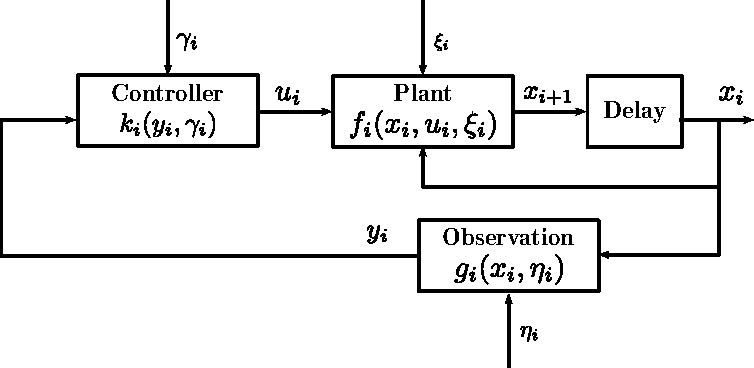
\includegraphics[scale=0.9]{plant_dist.pdf}  \\
    \caption{Schematic diagram of general stochastic control system.}
    \label{fig:gen_plant}
\end{figure}

The formulation of the optimal control used in this work requires a particular stochastic differential equation using \textbf{Brownian motion}, also known as \textbf{Wiener Process}. According to \citep{kappen2011optimal}, this process presents a Gaussian conditional likelihood with a variance that increases linearly in the time interval and has zero mean. Therefore, in order to the following differential equation to be valid, it needs to satisfy $\langle\dif \xi \dif \xi \rangle = v_{ij}\dif t$, where $v$ is a symmetric positive definite matrix.

\begin{equation}
    \dif x = f(x(t),u(t),t)\dif t + \dif \xi
    \label{eq:st_diff}
\end{equation}

For instance, if the state variable in equation \ref{eq:st_diff} is a single state, with means the value of $v$ is a positive scalar, we have: 
\begin{equation}
    x_{t+1} = x_t + \xi, \quad \xi_t = \pm\sqrt{v}
    \label{eq:st_diff_1}
\end{equation}
Then, the conditional probability distribution of $x$ at time $t$ given initial condition is Gaussian and specified by its mean and variance. 
\begin{equation}
\rho\left(x, t \mid x_{0}, 0\right)=\frac{1}{\sqrt{2 \pi \nu t}} \exp \left(-\frac{\left(x-x_{0}\right)^{2}}{2 \nu t}\right)
\end{equation}


\section{Stochastic Optimal Control}
As already stated in the previous section, optimal control formulation's main objective is to drive the states to another state that obeys an objective goal, which can also be found in control engineering literature, as cost function, performance measurement, and others. For instance, if the objective goal is defined to track reference states of a continuous-time system with no perturbation, it can be mathematically described as in the following:

\begin{equation}
\begin{aligned}
J(x,t) = \min_{u} \quad & (x-\bar{x})^2\\
\textrm{s.t.} \quad & \dot{x}=f(x,u,t)\\
\end{aligned}
\end{equation}
where $\bar{x}$ is the desired trajectory of the states. Therefore, the goal is to find an optimal solution to control input that drives the states $x$ to $\bar{x}$. The solution to this optimal problem has been solved by different methods \citep{kirk2004optimal}. However, there are uncertainties for the Stochastic system that would result in a slightly different cost function. 

The cost function to find an optimal control solution of control input is defined in equation \ref{eq:cost}, which corresponds to the previous stochastic dynamic system's expectation. 
\begin{equation}
J(t,x) = \: \mathbb{E}_{\mathbb{Q}}\left[\phi\left(\mathrm{x}_{T}, T\right)+\int_{t_{0}}^{T} \mathrm{R}\left(\mathrm{x}_{t},\mathrm{u}_{t}, t\right) \mathrm{d} t\right]
\label{eq:cost}
\end{equation}

where the \textit{end cost} $\phi\left(\mathrm{x}_{T}, T\right)$ gives the penalty to the last state configuration and integral term is the cost associate to the trajectories $x(0\longmapsto T)$, also known as \textit{optimal cost to go}. 

\subsection{Hamilton-Jacobi-Bellman (HJB) solution}

It is necessary to perform a partial derivative (Taylor series expansion) of the cost function with respect to $\dif x$ and $\dif t$ to obtain the Stochastic Hamilton-Jacobi-Bellman (HJB) equation. Recalling that the stochastic system uses Wiener Process, the partial terms must expand up to order $\dif x^2$

\begin{equation}
\begin{aligned}
\left\langle J\left(t+d t, x_{t+\dif t}\right)\right\rangle &=\int \dif x_{t+\dif t} \mathcal{N}\left(x_{t+\dif t} \mid x_{t}, \nu \dif t\right) J\left(t+\dif t, x_{t+\dif t}\right) \\
&=J\left(t, x_{t}\right)+\dif t \partial_{t} J\left(t, x_{t}\right)+\langle \dif x\rangle \partial_{x} J\left(t, x_{t}\right)+\frac{1}{2}\left\langle \dif x^{2}\right\rangle \partial_{x}^{2} J\left(t, x_{t}\right) \\
\langle \dif x\rangle &=f(x, u, t) \dif t \\
\left\langle \dif x^{2}\right\rangle &=\nu(t, x, u) \dif t
\end{aligned}
\end{equation}

Therefore the resulting Stochastic HJB equation is giving in the following:

\begin{equation}
-\partial_{t} J(t, x)=\min _{u}\left(R(t, x, u)+f(x, u, t) \partial_{x} J(x, t)+\frac{1}{2} \nu(t, x, u) \partial_{x}^{2} J(x, t)\right) \label{eq:hjb}
\end{equation}

where the boundary condition is $F(x,T) = \phi(x)$.

Therefore, the optimal control input is the solution of Equation \ref{eq:hjb}. When $v \longmapsto 0$, the Stochastic HJB reduces to a deterministic HJB problem \citep{kappen2011optimal}. The traditional approach for solving linear problems are based on Ricatti equations \citep{kirk2004optimal}.

\subsection{Path Integral Control} \label{se:path} The solution of a stochastic optimization problem for a linear system, being discrete or continuous, can be easily solved by Riccati equations \citep{kirk2004optimal}. However, a solution for nonlinear is not possible. By transforming the performance measurement (cost function) into an expectation over all possible trajectories, the solution can be obtained with Monte Carlo approximation using forward sampling \citep{kappen2005path}. The transformation of the cost function is performed with FeynmanKac lemma, which maps the parabolic partial differential equations (PDEs) to a path integral representation \citep{theodorou2010generalized}. 

Before presenting the path integral control solution for stochastic system, the full dynamic system presented in Figure \ref{fig:gen_plant} is defined in the following using Brownian disturbance:

%In general the HJB is impossible to solve analytically, and numerical solutions are intractable due to the curse of dimensionality. One way to proceed is to consider the class of control problems in which the HJB can be linearized, and, consequently, expressed as a path integral [2]. Using this approach, researchers have developed computationally efficient methods that have been successfully applied to control, for example, cart-pole, multi agent systems like swarm of quadrotors, and RC Cars [10].

\begin{equation}
\dif x=\left[f\left(x_{t}, t\right)+G\left(x_{t}, t\right] u\left(x_{t}, t\right)\right) d t+B\left(x_{t}, t\right) \dif w
\end{equation}

The cost function also contains a quadratic control cost to minimize the control input, as defined in the following. Note the matrix $R$ must be a positive definite matrix.

\begin{equation}
\mathbf{u}^{*}(\cdot)=\underset{\mathfrak{u} (\cdot)}{\operatorname{arg min}} \: \mathbb{E}_{\mathbb{Q}}\left[\phi\left(\mathrm{x}_{T}, T\right)+\int_{t_{0}}^{T} \mathcal{L}\left(\mathrm{x}_{t}, \mathbf{u}_{t}, t\right) \mathrm{d} t\right]
\label{eq:cost}
\end{equation}
Noting that: 
\begin{equation}
\mathcal{L}\left(\mathrm{x}_{t}, \mathbf{u}_{t}, t\right)=q\left(\mathrm{x}_{t}, t\right)+\frac{1}{2} \mathbf{u}_{t}^{\mathrm{T}} \mathbf{R}\left(\mathrm{x}_{t}, t\right) \mathbf{u}_{t}
\end{equation} 
where the \textit{end cost} $\phi\left(\mathrm{x}_{T}, T\right)$ gives the penalty to the last state configuration and $\mathcal{L}\left(\mathrm{x}_{t}, \mathbf{u}_{t}, t\right)$ is the cost associate to the trajectories $x(0\longmapsto T)$, also known as \textit{optimal cost to go}. 

In order to estimate how the probability distribution from the uncontrolled $\mathbb{P}$ and controlled $\mathbb{Q}$ dynamics, it is used the Girsanov's theorem \citep{girsanov1960transforming}. This is called as relative entropy. 

\begin{equation}
\mathrm{D}_{K L}(\mathbb{Q}(\mathbf{u}) \| \mathbb{P}) =  \frac{1}{2} \int_{t_{0}}^{T} \mathbf{u}_{t}^{\mathrm{T}} \mathbf{G}\left(\mathrm{x}_{t}, t\right)^{\mathrm{T}} \left[B\left(x_{t}, t\right)B\left(x_{t}, t\right)^T\right]^{-1} \mathbf{G}\left(\mathrm{x}_{t}, t\right) \mathbf{u}_{t} \mathrm{~d} t \label{eq:entropy}
\end{equation}

Defining $\Sigma\left(\mathrm{x}_{t}, t\right) = B\left(x_{t}, t\right)B\left(x_{t}, t\right)^T$, and assuming $\mathbf{R}$ is the product of a scalar positive value $\lambda$ and $\mathbf{G}\left(\mathrm{x}_{t}, t\right)^{\mathrm{T}} \Sigma\left(\mathrm{x}_{t}, t\right)^{-1} \mathbf{G}\left(\mathrm{x}_{t}, t\right)$, we can re-write equation \ref{eq:entropy} as:

\begin{equation}
\begin{split}
\mathrm{D}_{K L}(\mathbb{Q}(\mathbf{u}) \| \mathbb{P}) &=  \frac{1}{2} \int_{t_{0}}^{T} \mathbf{u}_{t}^{\mathrm{T}} \mathbf{G}\left(\mathrm{x}_{t}, t\right)^{\mathrm{T}} \Sigma\left(\mathrm{x}_{t}, t\right)^{-1} \mathbf{G}\left(\mathrm{x}_{t}, t\right) \mathbf{u}_{t} \mathrm{~d} t \\
&=  \frac{1}{2} \int_{t_{0}}^{T} \mathbf{u}_{t}^{\mathrm{T}} \lambda \mathbf{R}\ \mathbf{u}_{t} \mathrm{~d} t
\end{split}
\end{equation}

Therefore, the cost function presented in equation \ref{eq:cost}, can be written as:

\begin{equation}
\mathbb{E}_{\mathbb{Q}}\left[\phi\left(\mathrm{x}_{T}, T\right)+\int_{t_{0}}^{T} \mathcal{L}\left(\mathrm{x}_{t}, \mathbf{u}_{t}, t\right) \mathrm{d} t\right] = 
\mathbb{E}_{\mathbb{Q}}\left[\phi\left(\mathrm{x}_{T}, T\right)+\lambda\mathrm{D}_{K L}(\mathbb{Q}(\mathbf{u}) \| \mathbb{P}) \right] 
\end{equation}

The path integral expression presented in the following is the contribution of the relationship between Free Energy and Relative Entropy, which is proof by \citep{theodorou2015nonlinear}.

\begin{equation}
-\lambda \mathcal{F}(S(\tau))=\inf _{\mathbb{Q}}\left[\mathrm{E}_{\mathbb{Q}}[S(\tau)]+\lambda \mathbb{D}_{K L}(\mathbb{Q} \| \mathbb{P})\right] \label{eq:pathint}
\end{equation}

where $\mathcal{F}(S(\tau))$ is the free energy distribution over $\phi\left(\mathrm{x}_{T}, T\right)/\lambda$: 

\begin{equation}
    \mathcal{F}(S(\tau)) = \textrm{log}\left( 
    \mathbb{E}_{\mathbb{Q}}\left[\textrm{exp}\left(-\frac{1}{\lambda}\phi\left(\mathrm{x}_{T}, T\right)\right)\right]\right) 
\end{equation}

According to \citet{theodorou2015nonlinear}, the infimum of the equation \ref{eq:pathint} at differentiation of optimal probability measured of controlled dynamics $\mathbb{Q}^*$ with respect to probability measure of uncontrolled dynamics $\mathbb{P}^*$ is: 

\begin{equation}
\frac{\mathrm{d} \mathbb{Q}^{*}}{\mathrm{~d} \mathbb{P}}=\frac{\exp \left(-\frac{1}{\lambda} S(\tau)\right)}{\mathbb{E}_{\mathbb{P}}\left[\exp \left(-\frac{1}{\lambda} S(\tau)\right)\right]}
\label{eq:opprQ}
\end{equation}

Therefore, the computation of the stochastic HJB equation can be avoid by using the relative entropy between $\mathbb{Q}^*$, as stated in \citep{williams2016aggressive}:

\begin{equation}
\mathbf{u}^{*}(\cdot)=\operatorname{argmin}_{\mathbf{u}(\cdot)} \mathbb{D}_{K L}\left(\mathbb{Q}^{*} \| \mathbb{Q}(\mathbf{u})\right)
\end{equation}

The formulation of entropy minimization is described in Appendix \ref{appendix-customize-this-label} and detailed explained in \citep{williams2016aggressive}. Therefore, the resultant entropy is:

\begin{equation}
\begin{aligned}
\mathcal{D}(\tau, \mathbf{u}(\cdot))=&-\int_{0}^{T} \mathbf{u}_{t}^{\mathrm{T}} \mathrm{G}\left(\mathrm{x}_{t}, t\right)^{\mathrm{T}} \Sigma\left(\mathrm{x}_{t}, t\right)^{-1} \mathbf{B}\left(\mathrm{x}_{t}, t\right) d w^{(0)} \\
&+\frac{1}{2} \int_{0}^{T} \mathbf{u}_{t}^{\mathrm{T}} \mathbf{G}\left(\mathrm{x}_{t}, t\right)^{\mathrm{T}} \Sigma\left(\mathrm{x}_{t}, t\right)^{-1} \mathbf{G}\left(\mathrm{x}_{t}, t\right) \mathbf{u}_{t} \mathrm{~d} t
\end{aligned}
\end{equation}

In conclusion, for a discrete time the optimal control is defined as : 

\begin{equation}
\mathbf{u}_{j}^{*}= \frac{1}{\Delta t} \mathrm{E}_{\mathbb{P}}\left[\frac{\exp \left(-\frac{1}{\lambda} S(\tau)\right) \mathcal{H}\left(\mathrm{x}_{t_{j}}, t_{j}\right)}{\mathbb{E}_{\mathbb{P}}\left[\exp \left(-\frac{1}{\lambda} S(\tau)\right)\right]}\right]^{-1} \mathbb{E}_{\mathbb{P}}\left[\frac{\exp \left(-\frac{1}{\lambda} S(\tau)\right) \mathcal{G}\left(\mathrm{x}_{t_{j}}, t_{j}\right) \epsilon_{j} \sqrt{\Delta t}}{\mathrm{E}_{\mathbb{P}}\left[\exp \left(-\frac{1}{\lambda} S(\tau)\right)\right]}\right] \label{eq:uj}
\end{equation}

where,

\begin{equation}
\begin{aligned}
\mathcal{G}(\mathrm{x}, t) &=\mathbf{G}(\mathrm{x}, t)^{\mathrm{T}} \Sigma(\mathrm{x}, t)^{-1} \mathbf{B}(\mathrm{x}, t) \\
\mathcal{H}(\mathrm{x}, t) &=\mathrm{G}(\mathrm{x}, t)^{\mathrm{T}} \Sigma(\mathrm{x}, t)^{-1} \mathrm{G}(\mathrm{x}, t)
\end{aligned}\label{eq:GH}
\end{equation}


\section{Simulations}

The previous section described the stochastic dynamic system's description using Wiener Process and stabilized the optimization control formulation. The critical take-away is the definition of the control law expressed in equations \ref{eq:uj} and \ref{eq:GH}.

To apply this controller, researchers have been exploring various implementation algorithms, such as  Monte-Carlo sampling, to compute the control for the current state \citep{kappen2005path} and others. This work takes advantage of an extension of optimal control, called Model predictive control (MPC) \citep{richter2011advanced}. MPC is not a specific control strategy. However, it is the artifact to find the control input considering the concept of prediction by minimizing a cost function considering future error and constraints of the problem. See Appendix \ref{appendix-customize-this-label2} for the MPC algorithm used with Path Integral.

The proposed stochastic optimal control is implemented in two system: an inverted pendulum on a cart and a planar two-link robotic arm. The objective goal is to find an optimal control solution to drive the states into a vertical configuration then balance.

Both applications contain perturbation $\gamma_i$ in the control input as: 

\begin{equation}
\begin{split}
    E(\gamma_i)&=0\\
    E(\gamma_i)&=\delta_i^2 \quad 0 \leqslant i \leqslant N-1 
\end{split}
\end{equation}

Figure \ref{fig:pdf} shows the probability density function for the system's random uncertainty. The histogram contains the actual perturbation in the system. Kernel smoothing plot is an estimation of the pdf given the random variables. Last, the pdf plot (in yellow) corresponds to the pdf with a provided variance and mean. 

\begin{figure}[H]
\centering
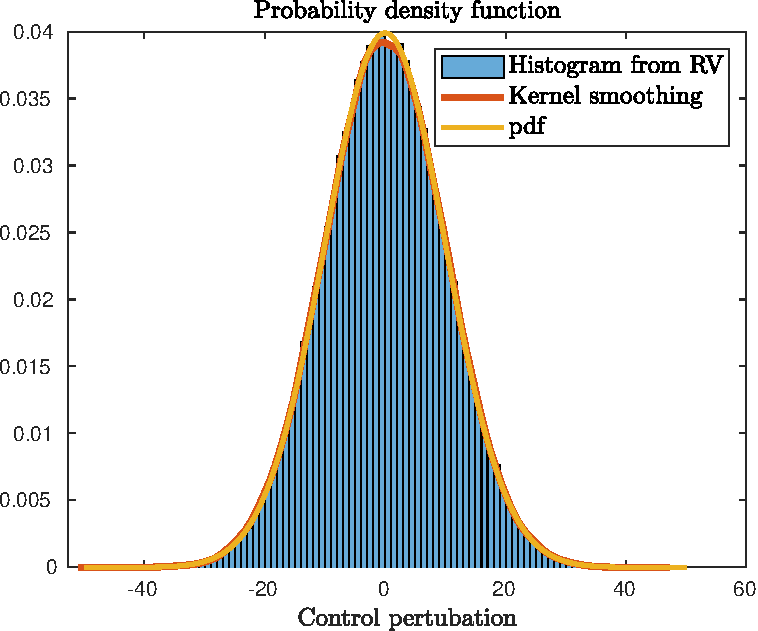
\includegraphics[width=0.6\textwidth]{pdf}
\caption{\label{fig:pdf}Probability density function.}
\end{figure}

\subsection{Inverted Pendulum on a cart}
A well-known problem in control theory is presented in the following to illustrate the contraction and introduce the stochastic optimal control solution of this work: the inverted pendulum problem. Figure \ref{fig:car_pole} consists of a motorized cart and a bar. The mathematical description of the problem is analog to technologies found on a rocket launch \citep{ogata2010modern} and two-wheeled self-balancing personal transporter \citep{chan2013review}. 
The governing equation is represented in \ref{eq:car_pole}:

\begin{figure}[H]
    \centering
    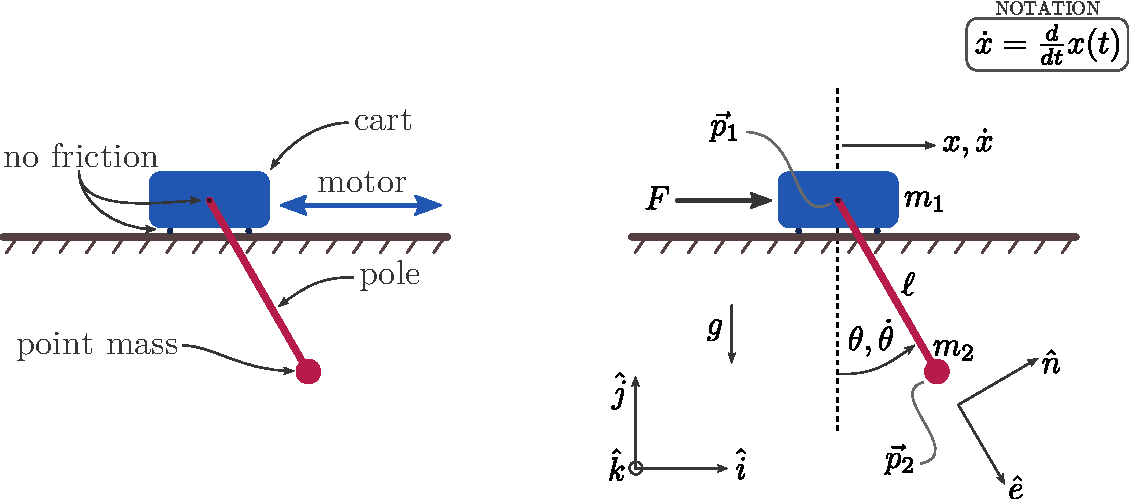
\includegraphics[scale=0.75]{cartPoleEqns.pdf} \\
    \caption{Inverted Pendulum System.}
    \label{fig:car_pole}
\end{figure}

The control input $u$ is the force $F$ that moves the cart, and the outputs are the angular position $\theta$ and the horizontal position of the cart $x$. For the optimal control formulation presented in this work, the author uses a state-space presentation, where the states are  $x=\begin{bmatrix} x & \dot{x} & \theta & \dot{\theta} \end{bmatrix} $. In control engineering, it corresponds to a system's mathematical model as a set of input, output, and state variables related by first-order differential equations.

\begin{equation}
\left(\begin{array}{cc}
\cos \theta & \ell \\
m_{1}+m_{2} & m_{2} \ell \cos \theta
\end{array}\right)\left(\begin{array}{l}
\ddot{x} \\
\ddot{\theta}
\end{array}\right)=\left(\begin{array}{c}
-g \sin \theta \\
F+m_{2} \ell \dot{\theta}^{2} \sin \theta
\end{array}\right) 
\label{eq:car_pole}
\end{equation}

The results of stochastic optimization control is presented in Figures \ref{fig:car_poleopt}, \ref{fig:car_poleopt2}, and \ref{fig:car_poleopt3}. The plot on the left shows the initial state. The plot on the right shows the final state. The plot in between shows an intermediate step to achieve the objective control. The curve presents the path of the endpoint. Note that the control input is only the trust force of the card. 

\begin{figure}[H]
    \centering
    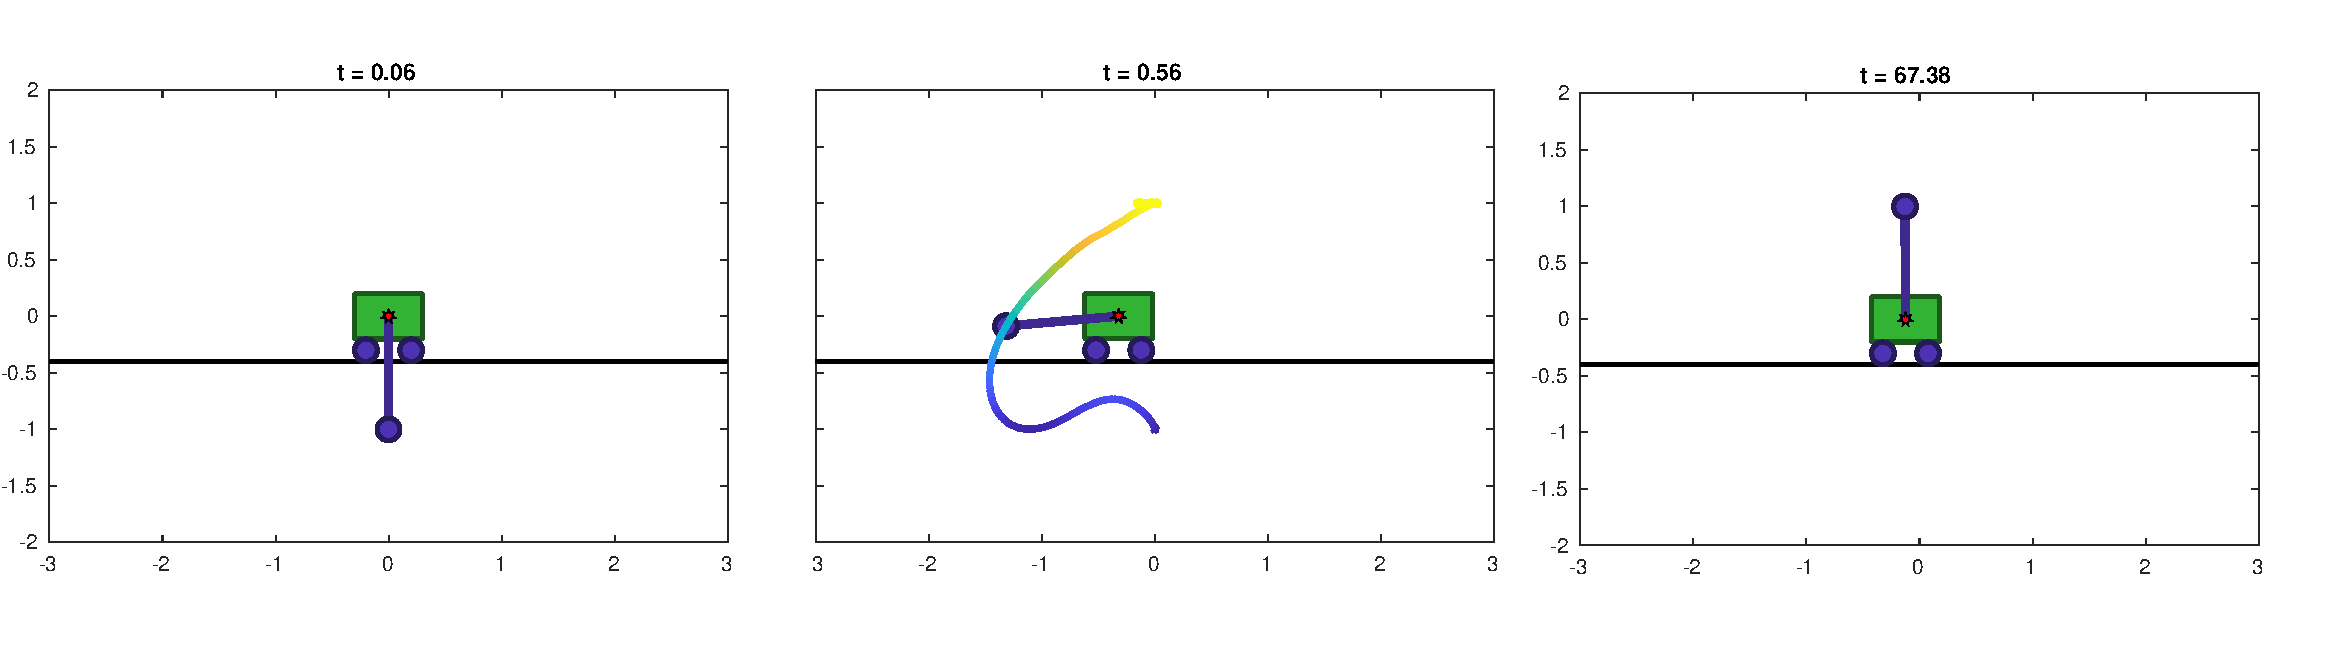
\includegraphics[width=1\textwidth]{pengulum_cart.pdf} \\
    \caption{Optimal trajectory for the Inverted Pendulum System on a cart.}
    \label{fig:car_poleopt}
\end{figure}

\begin{figure}[H]
\centering
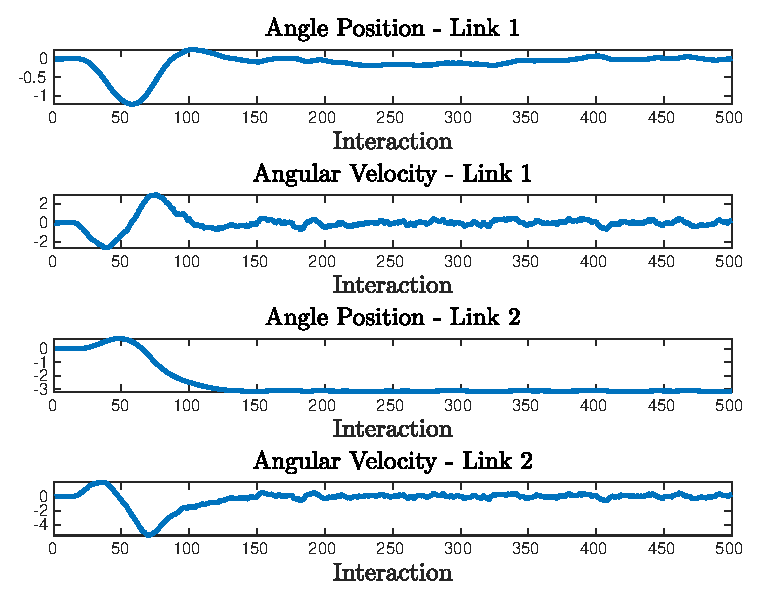
\includegraphics[width=0.6\textwidth]{states2}
\caption{State Space Results}
\label{fig:car_poleopt2}
\end{figure}

\begin{figure}[H]
\centering
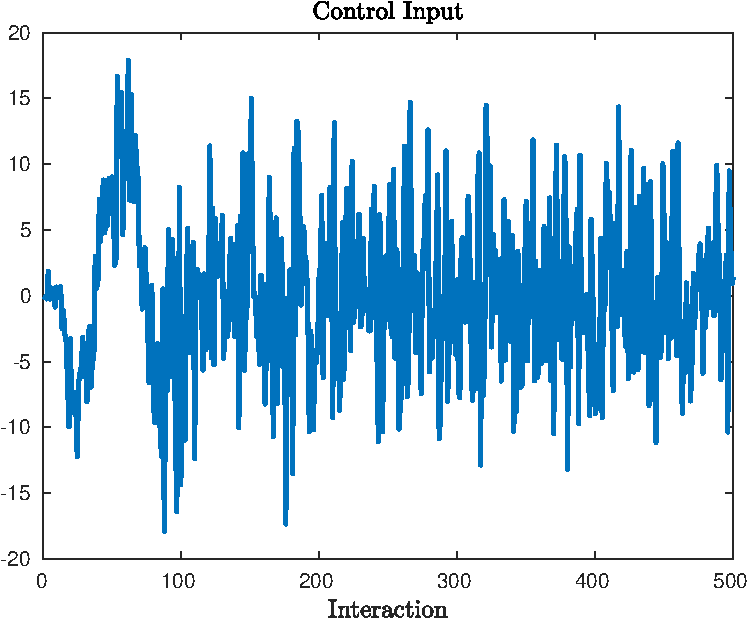
\includegraphics[width=0.6\textwidth]{control2}
\caption{Optimal Control solutions.}
\label{fig:car_poleopt3}
\end{figure}

\subsection{Planar two-link robotic arm} 

A planar two-link robotic arm, also know as acrobot, is composed of two rigid links connected by a two-degree rotational joint. In the control engineering literature, the common control task studied for this robot configuration is the swing-up task, aiming to find an optimal control solution to move the system into a vertical configuration then balance.

\begin{figure}[H]
    \centering
    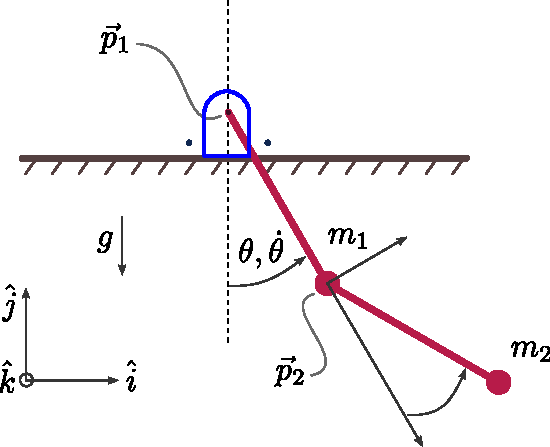
\includegraphics[scale=0.75]{cartPoleEqns (copy).pdf} \\
    \caption{Planar two-link robotic arm.}
    \label{fig:car_pole}
\end{figure}

The governing equation of a two-link robotic arm might be represented in the standard robotic formulation \cite{tedrake2016underactuated}:

\begin{equation}
\mathbf{M}(\mathbf{q}) \mathbf{q}+\mathbf{C}(\mathbf{q}, \mathbf{q}) \mathbf{q}=\tau_{g}(\mathbf{q})+\mathbf{B} \mathbf{u}
\end{equation}

where: 

\begin{equation}
    \begin{aligned}
    \mathbf{M}(\mathbf{q})&=\left[\begin{array}{cc}
I_{1}+I_{2}+m_{2} l_{1}^{2}+2 m_{2} l_{1} l_{c 2} c_{2} & I_{2}+m_{2} l_{1} l_{c 2} c_{2} \\
I_{2}+m_{2} l_{1} l_{c 2} c_{2} & I_{2}
\end{array}\right] \\
\mathbf{C}(\mathbf{q}, \mathbf{q})&=\left[\begin{array}{cc}
-2 m_{2} l_{1} l_{c 2} s_{2} \dot{q}_{2} & -m_{2} l_{1} l_{c 2} s_{2} q_{2} \\
m_{2} l_{1} l_{c 2} s_{2} \dot{q}_{1} & 0
\end{array}\right] \\
\tau_{g}(\mathbf{q})&=\left[\begin{array}{c}
-m_{1} g l_{c 1} s_{1}-m_{2} g\left(l_{1} s_{1}+l_{c 2} s_{1+2}\right) \\
-m_{2} g l_{c 2} s_{1+2}
\end{array}\right] \\
\mathbf{B}&=\left[\begin{array}{l}0 \\1\end{array}\right]
    \end{aligned}
\end{equation}

Note, the presented governing equation is a continuous-time nonlinear dynamical system. Therefore, for this project's conclusion, a discretization of the system is performed, and random perturbation is added to control and parameters. 

\begin{figure}[H]
\centering
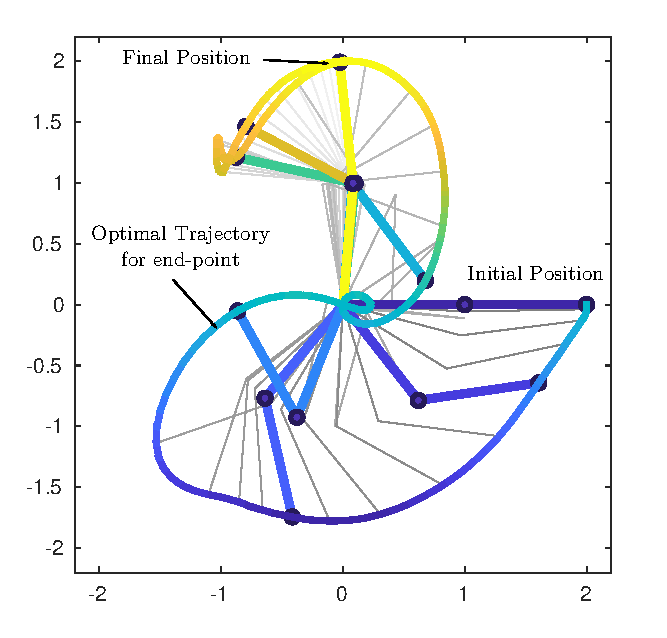
\includegraphics[width=0.7\textwidth]{acrobot.pdf}
\caption{Optimal trajectory for the planar two-link robotic arm.}
\label{fig:acrobot1}
\end{figure}

The optimal solution is presented in Figures \ref{fig:acrobot1}, \ref{fig:acrobot2}, and \ref{fig:acrobot3}. Figure \ref{fig:acrobot1} shows some snapshots during animation of the swing-up maneuver. Note, the robot starts with the joints to the right, and it moves to the left to storage potential energy and moves up. 

\begin{figure}[H]
\centering
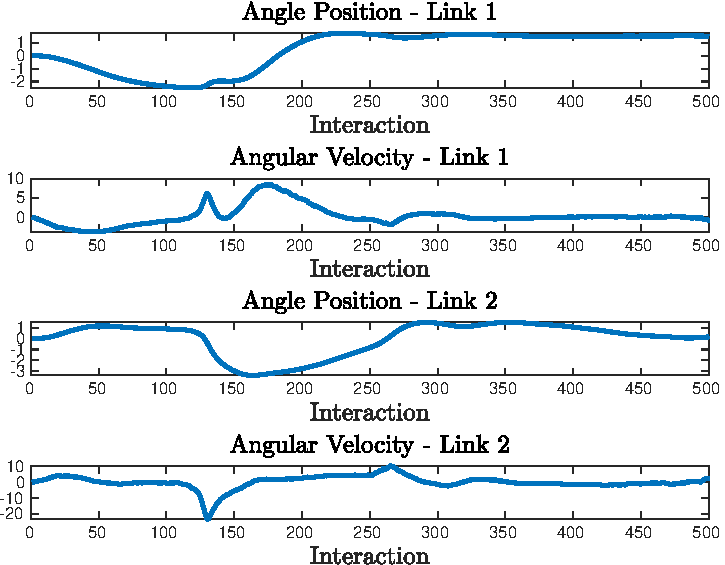
\includegraphics[width=0.6\textwidth]{states}
\caption{State Space Results}
\label{fig:acrobot2}
\end{figure}

\begin{figure}[H]
\centering
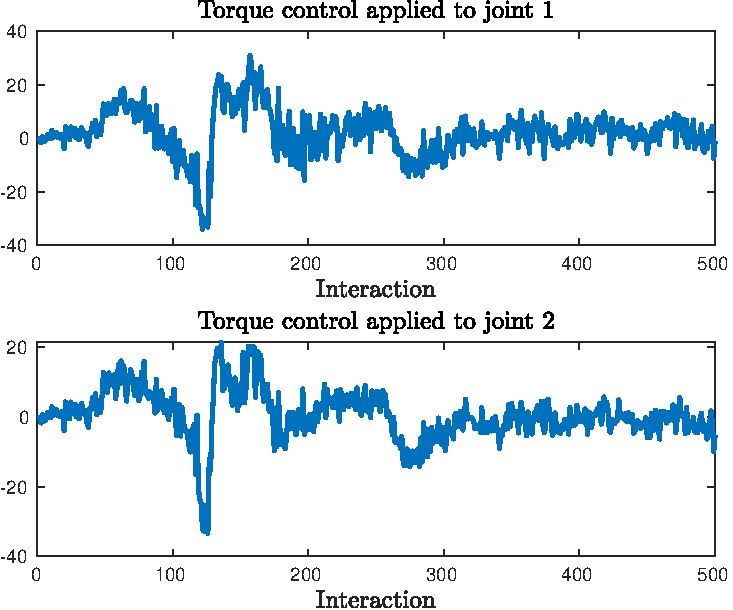
\includegraphics[width=0.6\textwidth]{control}
\caption{Optimal Control solutions.}
\label{fig:acrobot3}
\end{figure}

\section{Matlab Implementation}

All the code is available at: \url{https://github.com/EriveltonGualter/ESC-704-Stochastic-Systems}.

To compute the entered problem, run the \mcode{MAIN.m} file:

\begin{lstlisting}
run('MAIN.m')
\end{lstlisting}

Otherwise, if it is desired only show the plots, run the MAINPresentation.m file:

\begin{lstlisting}
run('MAIN_Presentation.m')
\end{lstlisting}



% These commands need to appear at the point where you want
% the first page to end.
\restoregeometry
\newgeometry{bottom=0.5in}

%Begin appendix section(s)
\appendix

% Add appendices here:
\section{Relative Entropy Minimization}
\label{appendix-customize-this-label}

The optimal control solution using path integral method has been greatly presented in \citet{williams2016aggressive} and here is just described the high level derivations.

First, it is found the relative entropy between the optimal distribution $\textbb{Q}^*$ and induced distribution $\textbb{Q}(\textbb{u})$ of the control:
\begin{equation}
\mathbb{D}_{K L}\left(\mathbb{Q}^{*} \| \mathbb{Q}(\mathrm{u})\right)=\mathbb{E}_{\mathbb{Q}} *\left[\log \left(\frac{\mathrm{d} \mathbb{Q}^{*}}{\mathrm{~d} \mathbb{Q}(\mathbf{u})}\right)\right]
\end{equation}

After applying the chain rule property of Radon-Nikodym derivatives and Girsanov's theorem, we have:

%\begin{equation}
%\frac{\mathrm{d} \mathbb{Q}^{*}}{\mathrm{~d} \mathbb{Q}(\mathbf{u})}=\frac{\mathrm{d} %%\mathbb{Q}^{*}}{\mathrm{~d} \mathbb{P}} \frac{\mathrm{d} \mathbb{P}}{\mathrm{d} \mathbb{Q}(\mathbf{u})}
%\end{equation}

where $\frac{\mathrm{d} \mathbb{P}}{\mathrm{d} \mathbb{Q}(\mathbf{u})}$ is defined as:

\begin{equation}
\frac{\mathrm{d} \mathbb{P}}{\mathrm{d} \mathbb{Q}(\mathbf{u})}=\exp (\mathcal{D}(\tau, \mathbf{u}(\cdot)))
\end{equation}

and 

\begin{equation}
\begin{aligned}
\mathcal{D}(\tau, \mathbf{u}(\cdot))=&-\int_{0}^{T} \mathbf{u}_{t}^{\mathrm{T}} \mathrm{G}\left(\mathrm{x}_{t}, t\right)^{\mathrm{T}} \Sigma\left(\mathrm{x}_{t}, t\right)^{-1} \mathbf{B}\left(\mathrm{x}_{t}, t\right) d w^{(0)} \\
&+\frac{1}{2} \int_{0}^{T} \mathbf{u}_{t}^{\mathrm{T}} \mathbf{G}\left(\mathrm{x}_{t}, t\right)^{\mathrm{T}} \Sigma\left(\mathrm{x}_{t}, t\right)^{-1} \mathbf{G}\left(\mathrm{x}_{t}, t\right) \mathbf{u}_{t} \mathrm{~d} t
\end{aligned}
\end{equation}

Combining with equation \ref{eq:opprQ}, the entropy between the optimal distribution $\textbb{Q}^*$ and probability distribution from the uncontrolled dynamics $\textbb{P}$ is defined as:

\begin{equation}
\mathbb{D}_{K L}\left(\mathbb{Q}^{*} \| \mathbb{Q}(\mathbf{u})\right)=\mathbb{E}_{\mathbb{Q}^{*}}\left[\log \left(\frac{\exp \left(-\frac{1}{\lambda} S(\tau)\right) \exp (\mathcal{D}(\tau, \mathbf{u}(\cdot)))}{\mathbb{E}_{\mathbb{P}}\left[\exp \left(-\frac{1}{\lambda} S(\tau)\right)\right]}\right)\right.
\end{equation}

From section \ref{se:path}, the free energy distribution over $\phi\left(\mathrm{x}_{T}, T\right)/\lambda$, which correspond to the \textit{end cost}, does not depend of control. Therefore, the terms regarding this cost might be neglected. The minimization problem results in:

\begin{equation}
\underset{\mathfrak{u}(\cdot)}{\operatorname{argmin}} \:\: \mathbb{D}_{K L}\left(\mathbb{Q}^{*} \| \mathbb{Q}(\mathbf{u})\right)=\underset{\mathfrak{u}(\cdot)}{\operatorname{argmin}} \mathrm{E}_{\mathbb{Q}^{*}}[\mathcal{D}(\tau, \mathbf{u}(\cdot))]
\end{equation}


\newpage

\section{Model Predictive path integral control algorithm}
\label{appendix-customize-this-label2}

The MPC control works differently from the conventional controllers. Instead of controlling the plant-based in trying to minimize the past error, it simulates a series of candidate control inputs in the short future, which minimizes the desired cost function. When combining with scholastic optimal control formulation, the algorithm can be described in Figure \ref{fig:mpc} \citep{williams2016aggressive}.

\begin{figure}[H]
    \centering
    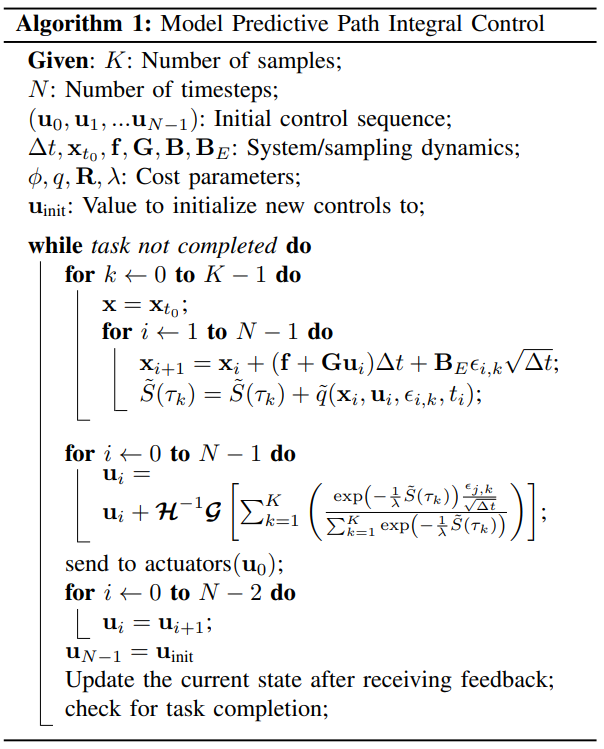
\includegraphics[scale=0.4]{mpc.png} \\
    \caption{MPC-Path Integral.}
    \label{fig:mpc}
\end{figure}

\newpage

% All references should be stored in the file "references.bib"
% Please do not modify anything below this line.
\printbibliography


\end{document}
